% This LaTeX was auto-generated from MATLAB code.
% To make changes, update the MATLAB code and export to LaTeX again.

\documentclass{article}

\usepackage[utf8]{inputenc}
\usepackage[T1]{fontenc}
\usepackage{lmodern}
\usepackage{graphicx}
\usepackage{color}
\usepackage{hyperref}
\usepackage{amsmath}
\usepackage{amsfonts}
\usepackage{epstopdf}
\usepackage[table]{xcolor}
\usepackage{matlab}

\sloppy
\epstopdfsetup{outdir=./}
\graphicspath{ {./Exercice1_images/} }

\begin{document}

\matlabheading{Exercice n°1 : Compensated Horner-Scheme}

\matlabheadingtwo{Question n°1 : classic horner scheme implementation}

\begin{matlabcode}
format long
p = [1 2 3 4 5 6 7 8 9];
x = pi;
res1 = polyval(p,x)
\end{matlabcode}
\begin{matlaboutput}
res1 = 
     2.041366687877934e+04

\end{matlaboutput}
\begin{matlabcode}
res2 = Horner (p,x)
\end{matlabcode}
\begin{matlaboutput}
res2 = 
     2.041366687877934e+04

\end{matlaboutput}


\matlabheadingtwo{Question n°2 and 3: EFT}

\begin{par}
\begin{flushleft}
Les fonctions sont disponibles en annexe 
\end{flushleft}
\end{par}

\begin{matlabcode}
res3 = CompHorner(p,x)
\end{matlabcode}
\begin{matlaboutput}
Unrecognized function or variable 'p'.
\end{matlaboutput}
\begin{matlabcode}
res4 = sHorner(p,x)
\end{matlabcode}


\matlabheadingtwo{Question n°4 : Symbolic math}

\begin{matlabcode}

n = 3:42;
x = 1.333
\end{matlabcode}
\begin{matlaboutput}
x = 1.3330
\end{matlaboutput}


\begin{matlabcode}
for i=1:length(n)
    a = poly(ones(1,n(i)));
    res1 = Horner    (a,x);     % Classic horner
    res2 = sHorner   (a,x);     % Thorical value
    res3 = CompHorner(a,x);     % Compensated Horner
    er1(i) = abs(res2-res1)/abs(res2);
    er2(i) = abs(res2-res3)/abs(res2);
    %c(i) = condp(a,x);
    c(i) = abs((x+1)/(x-1))^i;
    cond1(i) = 2*n(i)*eps*c(i);
    cond2(i) = eps + 4*n(i)*n(i)*eps*eps*c(i);
end
\end{matlabcode}


\begin{matlabcode}
cla
axis tight
figure(1)
loglog(c,er1,'b--d')
hold on;
loglog(c,er2,'r--x')
xlim([c(1) c(i)])
hold on
loglog(c,cond1)
hold on;
loglog(c,cond2)
hold on
xline(1/eps)
xline(1/(eps*eps))
\end{matlabcode}
\begin{center}
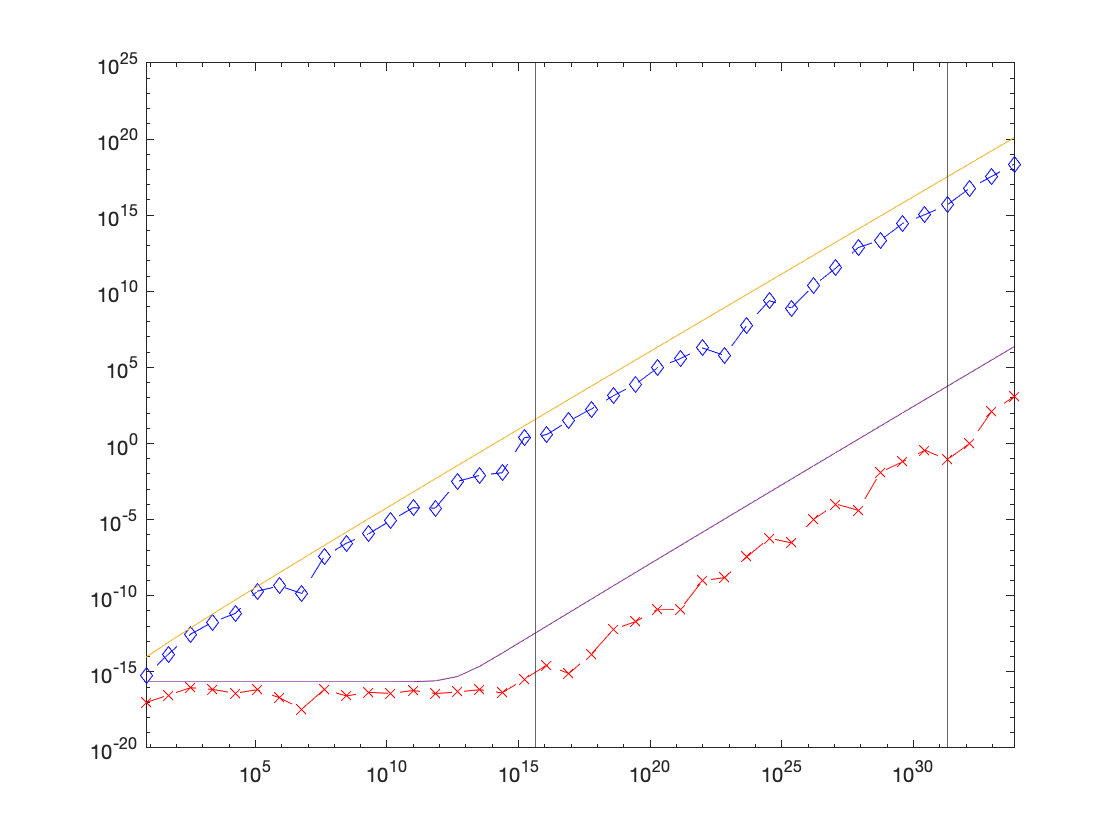
\includegraphics[width=\maxwidth{56.196688409433015em}]{figure_0.png}
\end{center}
\begin{matlabcode}



\end{matlabcode}

\end{document}
